\documentclass{article}
\usepackage[margin=0.5in]{geometry}
\usepackage[utf8]{inputenc}
\usepackage{graphicx}
\usepackage{hyperref}
\usepackage{color}
\usepackage{amsmath,amssymb}
\usepackage{algorithm}
\usepackage{algorithmic}

\title{UMass CMPSCI 383 (AI) HW3: Chapters 7-8}
\author{Answer Key}
\date{Assigned: Oct 6 2017; Due: Oct 13 2017 @ 11:55 PM EST}

\begin{document}

\maketitle

\begin{abstract}
    Submit a (.zip) file to Moodle containing your latex (.tex) file and rendered pdf. All written HW responses should be done in latex (use sharelatex.com or overleaf.com).
\end{abstract}

\section{Propositional Logic with Unicorns}
If the unicorn is mythical, then it is immortal, but if it is not mythical, then it is a mortal mammal. If the unicorn is either immortal or a mammal, then it is horned. The unicorn is magical if it is horned.

\subsection{Natural Language to Propositional Logic (15 pts)}

Translate the above statements into propositional logic using conjunctions ($\land$), disjunctions ($\lor$), implications ($\Rightarrow$), and negation ($\lnot$).

\begin{enumerate}
    \item Mythical $\Rightarrow$ Immortal 
    \item $\lnot$ Mythical $\Rightarrow$ $\lnot$Immortal $\land$  Mammal
    \item (Immortal $\lor$ Mammal) $\Rightarrow$ Horned
    \item Horned $\Rightarrow$ Magical
\end{enumerate}

\subsection{Propositional Logic to Conjunctive Normal Form (CNF) (15 pts)}
Convert the propositional logic statements into conjunctive normal form.

\begin{enumerate}
    \item $\lnot$Mythical $\lor$ Immortal
    \item (Mythical $\lor$ $\lnot$Immortal)  $\land$ (Mythical $\lor$ Mammal) 
    \item ($\lnot$Immortal $\lor$ Horned) $\land$ (Horned $\lor$ $\lnot$Mammal)
    \item $\lnot$Horned $\lor$ Magical
\end{enumerate}

\subsection{Apply the Resolution Method (30 pts)}
Your knowledge base (KB) consists of the 4 CNF statements you derived above. You can write your knowledge base as a conjunction ($\land$) of these statements. This should reveal a conjunction of 6 clauses. Write those clauses below.

\begin{enumerate}
    \item $\lnot$Mythical $\lor$ Immortal
    \item Mythical $\lor$ $\lnot$Immortal
    \item Mythical $\lor$ Mammal
    \item $\lnot$Immortal $\lor$ Horned
    \item Horned $\lor$ $\lnot$Mammal
    \item $\lnot$Horned $\lor$ Magical
\end{enumerate}

\noindent Now, use the resolution proof strategy to show that the unicorn is magical. Show your steps. You can either describe the resolution steps in words or you can use the diagram template at~\href{https://docs.google.com/drawings/d/1noR21Lkp1Hki2KK_N4lyy71ayVmQXB_O5x-d1EFviMg/edit?usp=sharing}{\color{blue}{HWs Public/HW2}} and include your figure (see Lecture 9, slides 8-17 for an example).

\begin{figure}
    \centering
    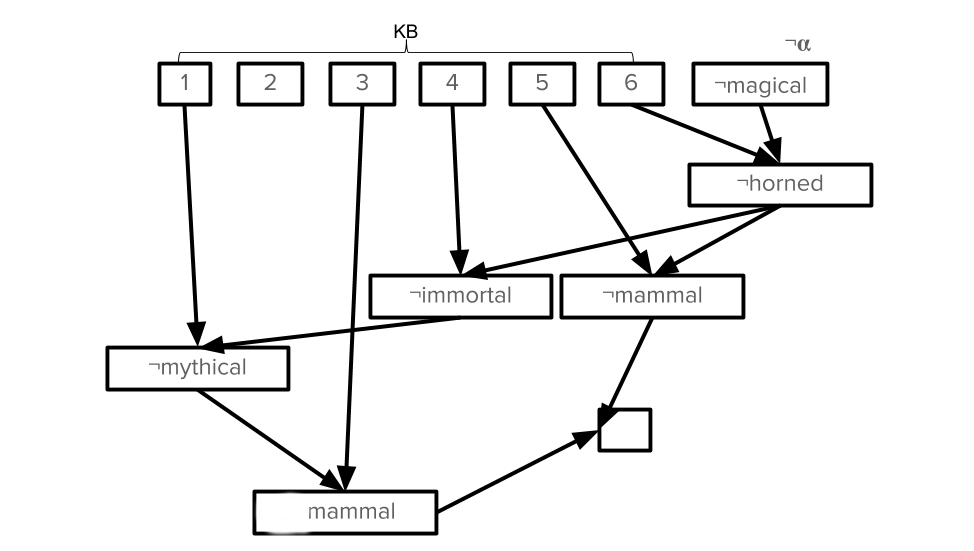
\includegraphics[scale=0.3]{figures/Resolution_Answer.png}
    \caption{Resolution Diagram}
    \label{fig:resolution}
\end{figure}

\section{Natural Language to First-Order Logic (20 pts)}
Write the following 6 statements and concepts in first-order logic. Make up reasonable predicates for each sentence.

\subsection{Every student who takes 383 wants an A.}
$\forall$ x In(x, CS383) $\Rightarrow$ WantsAnA(x)
\subsection{There is a barber who cuts the hair of all people in town who do not cut their own hair.}
$\exists$ x $\forall$ y $\lnot$cut(y, y) $\Rightarrow$ cut(x, y)
\subsection{Every year, it snows more in February than in April.}
$\forall$ x, y, z Year(z) $\land$isMonthOf(x, z) $\land$ isMonthOf(y, z) $\Rightarrow$ MoreSnow(x, y)
\subsection{No one in Amherst drives a Rolls-Royce.}
$\forall$x liveInAmherst(x) $\Rightarrow$ $\lnot$ driveRR(x)
\subsection{Grandchild}
$\forall$ GrandchildOf(x, y) $\Leftrightarrow$  ($\exists$p $\land$ ParentOf(x, p) $\land$ ParentOf(p, y))

\subsection{Brother}
$\forall$x, y Brother(x, y) $\Leftrightarrow$  $\exists$p $\lnot$ (x = y) $\land$ ParentOf(p, x) $\land$ ParentOf(p, y)
\subsection{SisterInLaw}
$\forall$x, y sisterInLawOf(x, y) $\Leftrightarrow$ $\lnot$(x = y) $\land$ $\exists$husband, spouse, $\lnot$(husband, spouse)$\land$ wifeOf(x,husband) $\land$ siblingOf(y, husband) $\lor$ sisterOf(x, spouse) $\land$ spouseOf(y, husband)
\subsection{Aunt}
$\forall$x, y Aunt(x, y) $\Leftrightarrow$ $\lnot$(x = y) $\land$ ($\exists$m, f, uncle $\lnot$(m = f)$\land$ $\lnot$(uncle = f)$\land$ $\lnot$(m = uncle)) $\land$ (sisterOf(x, m) $\lor$ sisterOf(x, f) $\lor$ wifeOf(uncle, x)
\section{Minesweeper}
Consider the minesweeper game in Lecture 8. Specifically, consider the game state below with the symbol names given in the adjacent figure.
\begin{figure}[h]
    \centering
    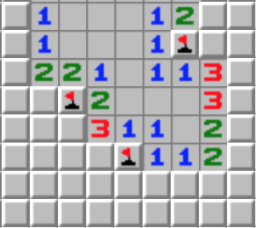
\includegraphics{figures/minesweeper.png}
    \hspace{1.0cm}
    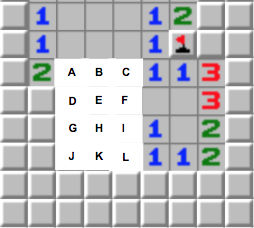
\includegraphics{figures/minesweeper_labels.png}
    \caption{Minesweeper}
    \label{fig:minesweeper}
\end{figure}

\subsection{a. (10 pts)} Following the example of Figure 7.5 in the text, construct the set of possible worlds (you should find 8 of them). Mark the worlds in which the KB is true and those in which each of the following sentences is true:

\begin{itemize}
    \item $\alpha_1$ = ``G Contains Bomb" \\
    \item $\alpha_2$ = ``J Does Not Contain A Bomb" \\
    \item $\alpha_3$ = ``K Does Not Contain A Bomb"
\end{itemize}

\noindent Assume G, J, and K can only take on the values True (i.e., "Contains Bomb") or False (i.e., "No Bomb"). All other observed variables can only take on their observed values. There is no need use graphics (as done in Figure 7.5), just list the worlds as a truth table.


\begin{table}[ht]
    \centering
    \begin{tabular}{c|c|c|c|c|c|c|c|c|c|c|c|c|c|c|c}
    A & B & C & D & E & F & G & H & I & J & K & L & KB & $\alpha_1$ & $\alpha_2$ & $\alpha_3$ \\ \hline
    2 & 1 & 0 & T & 2 & 0 & F & 3 & 1 & F & F & T & F & F & T & T\\ \hline
    2 & 1 & 0 & T & 2 & 0 & T & 3 & 1 & F & F & T & T & T & T & T\\ \hline
    2 & 1 & 0 & T & 2 & 0 & F & 3 & 1 & T & F & T & F & F & F & T\\ \hline
    2 & 1 & 0 & T & 2 & 0 & F & 3 & 1 & F & T & T & F & F & T & F\\ \hline
    2 & 1 & 0 & T & 2 & 0 & T & 3 & 1 & T & F & T & F & T & F & T\\ \hline
    2 & 1 & 0 & T & 2 & 0 & T & 3 & 1 & F & T & T & F & T & T & F\\ \hline
    2 & 1 & 0 & T & 2 & 0 & F & 3 & 1 & T & T & T & F & F & F & F\\ \hline
    2 & 1 & 0 & T & 2 & 0 & T & 3 & 1 & T & T & T & F & T & F & F
\end{tabular}
    \caption{Truth Table}
    \label{tab:my_label}
\end{table}

\subsection{b. (10pts)} Using the truth table, explain why model checking shows that KB $\models \alpha_1$, KB $\models \alpha_2$, and that KB $\models \alpha_3$.\\

$M(KB) = \{ \}$ \\
$M(\alpha_1) = \{ \}$ \\
$M(KB) \subseteq M(\alpha_1)$?

In this case, we need to proof that $M(KB) \subseteq M(\alpha_1)$. We know that $M(KB) = \{2\}$(In the second row, KB is correct) $M(\alpha_1) = \{2,5,6,8\}$(In the second, fifth, sixth, eighth rows, $\alpha_1$ are correct)
Since $M(KB) \subseteq M(\alpha_1)$, so KB $\models \alpha_1$

Same reason, in the second row of $\alpha_2, \alpha_3$ are true, and the second row of KB is the only true, so $M(KB) \subseteq M(\alpha_2)$ and $M(KB) \subseteq M(\alpha_3)$. So, KB $\models \alpha_2$, and KB $\models \alpha_3$.\\

\end{document}
